\section{VNA measurements and impedance transformation discussion} 

This section details the practical experiments conducted with the Vector Network Analyzer (VNA) and the assembly and testing of a Radio-Frequency Front-End (RFFE) receiver. 

\subsection{Impedance transformation with an L-Match network}

The L-Match network is a simple and effective way to match a source impedance to a load impedance using two reactive components, typically an inductor and a capacitor. In this section, we will analyze the performance of an L-Match network designed to match a source impedance of \( Z_0 = 50 \Omega \) to a load impedance of \( Z_L = 200 \Omega \), as shown in Figure \ref{fig:match_network}.

\begin{figure}[H]
    \centering
    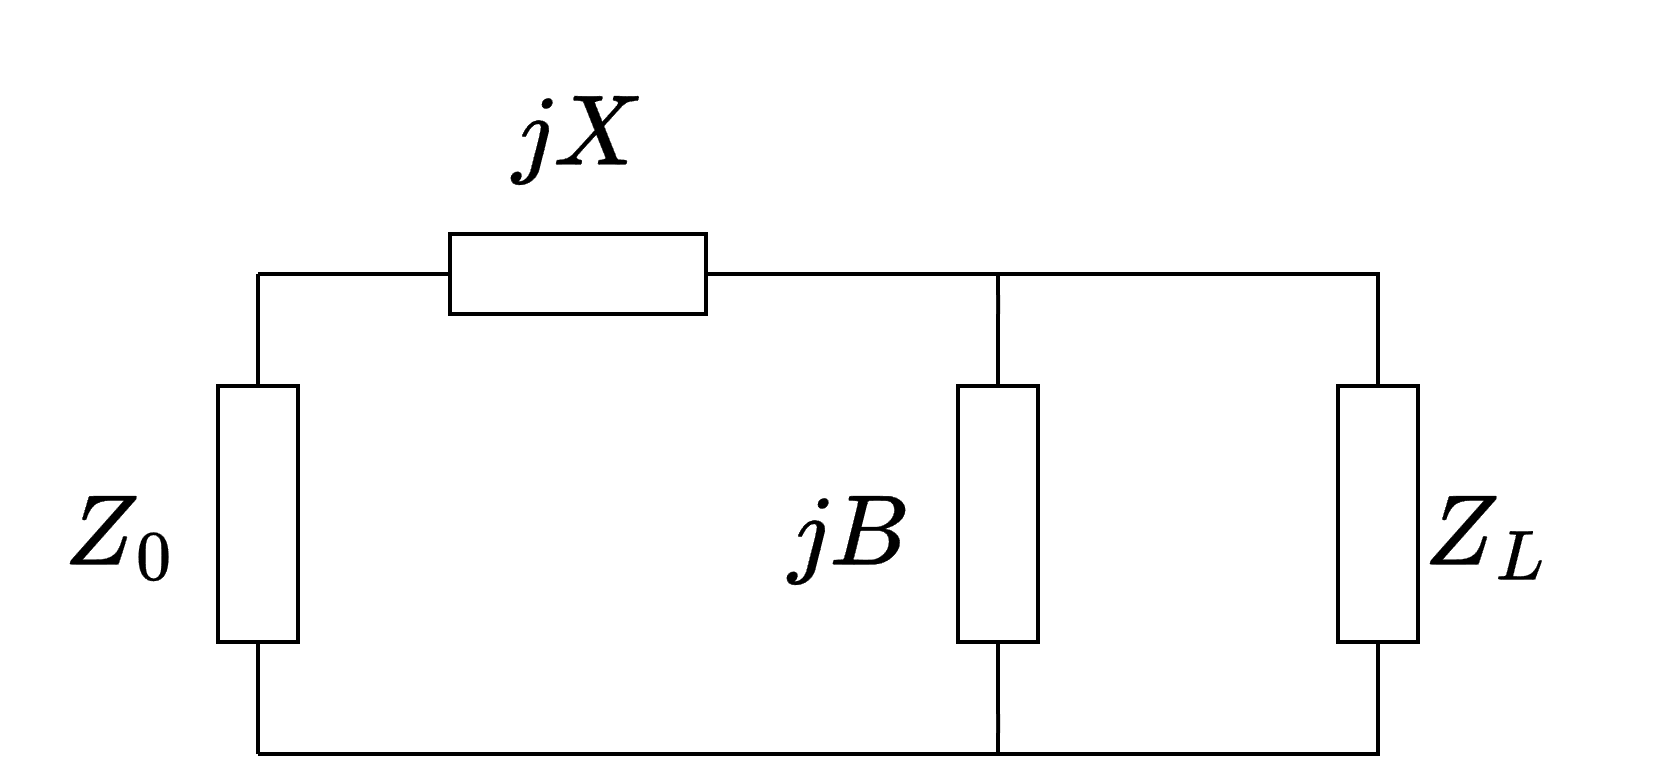
\includegraphics[width=0.5\textwidth]{Images/input-matching.png}
    \caption{L-Match Network for Impedance Transformation}
    \label{fig:match_network}
\end{figure}

\subsubsection{Theoretical Demonstration}
The L-Match network shown in Figure \ref{fig:match_network} is designed to transform a load impedance $Z_L$ into a desired input impedance $Z_{0}$. 

The total input impedance $Z_{0}$ is the sum of the series reactance $jX$ and the impedance of the parallel combination of $Z_L$ and $jB$\textsuperscript{\cite{Gillermo-Gonzalez}}:
$$Z_{0} = jX + (Z_L \parallel jB)$$

The impedance of the parallel portion ($Z_p$) is:
$$Z_p = \frac{Z_L \cdot (jB)}{Z_L + jB}$$

To simplify, we can rationalize this expression:
$$Z_p = \left( \frac{jB Z_L}{Z_L + jB} \right) \cdot \left( \frac{Z_L - jB}{Z_L - jB} \right) = \frac{jB Z_L^2 + B^2 Z_L}{Z_L^2 + B^2}$$

Separating the real ($R_p'$) and imaginary ($X_p'$) parts of $Z_p$:
$$Z_p = \underbrace{\left( \frac{Z_L B^2}{Z_L^2 + B^2} \right)}_{R_p'} + j \underbrace{\left( \frac{Z_L^2 B}{Z_L^2 + B^2} \right)}_{X_p'}$$

Now, substitute this back into the equation for $Z_{0}$:
$$Z_{0} = R_p' + jX_p' + jX_A = \left( \frac{Z_L B^2}{Z_L^2 + B^2} \right) + j \left( X + \frac{Z_L^2 B}{Z_L^2 + B^2} \right)$$

For a perfect impedance match, $Z_{0}$ must be purely resistive and equal to $R_{in}$ (e.g., $50 \Omega$). This imposes two conditions:

\begin{enumerate}
    \item \textbf{Real Part:} The real part of $Z_{0}$ must equal $R_{in}$.
    $$Z_{0} = \frac{Z_L B^2}{Z_L^2 + B^2}$$

    \item \textbf{Imaginary Part:} The imaginary part of $Z_{0}$ must be zero.
    $$X + \frac{Z_L^2 B}{Z_L^2 + B^2} = 0 \implies X= - \left( \frac{Z_L^2 B}{Z_L^2 + B^2} \right)$$
\end{enumerate}

These equations demonstrate that by choosing appropriate values for $X$ and $B$, the transformation is possible. Condition 2 shows that $X$ and $B$ must have opposite signs (one must be an inductor, the other a capacitor) for the reactances to cancel, leaving a purely resistive input.

\subsubsection{Design Example and Quality Factor}
